\documentclass[journal]{IEEEtran}
\usepackage[utf8]{inputenc}

\usepackage{hyperref}
\usepackage{graphicx}
\ifCLASSINFOpdf
\else
\fi
\usepackage{amsfonts}
\usepackage{color}
%\usepackage[dvipsnames]{xcolor}
\usepackage{soul}
\hyphenation{op-tical net-works semi-conduc-tor ns- however}
\usepackage{subfigure}
\usepackage{tabularx,booktabs}
\usepackage{amsmath,amssymb,amsfonts}
\usepackage{textcomp}
\usepackage{url}
\usepackage{multirow}
\newcommand{\cmark}{\ding{51}}%
\newcommand{\xmark}{\ding{55}}%
\usepackage[table,xcdraw]{xcolor}

\usepackage{boldline}
\usepackage{amssymb}
\usepackage{pifont}

\usepackage[noadjust]{cite}
\renewcommand{\citepunct}{,\penalty\citepunctpenalty\,}
\renewcommand{\citedash}{--}% optionally

\begin{document}

\title{Blockchain-enabled Network Sharing for O-RAN}

\author{Francesc~Wilhelmi~and~Lorenza~Giupponi%
\thanks{Francesc Wilhelmi and Lorenza Giupponi are with Centre Tecnol\`ogic de Telecomunicacions de Catalunya (CTTC/CERCA).}% <-this % stops a space
}

\maketitle

\begin{abstract}
The innovation provided by network virtualization in 5G, together with standardization and openess boosted by the Open Radio Access Network (O-RAN) Alliance, has paved the way to a collaborative future in communications systems, driven by flexible network sharing. Such advents are expected to attract new players like content providers and verticals, thus increasing competitiveness in the mobile market. However, scalability and trust issues are expected to arise, given the criticity of ownership traceability and resource exchanging in an open RAN sharing ecosystem. To address that, we propose the integration of Blockchain (BC) technology for enabling Mobile Network Operators (MNOs) and other players to exchange RAN resources (e.g., infrastructure, spectrum usage) autonomously and dynamically. BC will provide robustness, trustworthiness, and reliability to mobile networks, so that confidence is generated in an open RAN environment. In particular, we define a novel O-RAN-based BC-enabled architecture that allows automating RAN sharing procedures through either auction or marketplace-based mechanisms. The potential advantages of the proposed solution are demonstrated through simulation results. 
\end{abstract}

\begin{IEEEkeywords}
5G/6G, architecture, auction, blockchain, O-RAN, RAN sharing
\end{IEEEkeywords}

\IEEEpeerreviewmaketitle

%%%%%%%%%%%%%%%%%%%%%%%%%%%%
%% INTRODUCTION
%%%%%%%%%%%%%%%%%%%%%%%%%%%%
\section{Introduction}

As of today, 5G is a reality, with 100+ operators worldwide already deploying it. In spite of that, no matter the better capacity and latency offered by 5G, an increment in average revenue per user (ARPU) is unclear, and the past trends show that this indicator has been steadily decreasing for over a decade. An important aspect in the economics of 5G is that 70\% of network management costs are concentrated in the Radio Access Network (RAN)~\cite{ORAN2}. 

As a result there is currently and increasing interest to cut both Capital and Operational Expenditures (CAPEX and OPEX) and increase automation in that segment of the network. The CAPEX of 5G are expected to be important and include items like more spectrum, deployment of new antennas and equipment upgrade, large scale small-cell deployments to pursue the mmWave vision, etc., so that RAN sharing solutions take an increasing pivotal role. 

The economic sustainability of future networks has paved the way to three main trends in industry. First, evolving inside 3rd Generation Partnership Project (3GPP) and Next Generation Mobile Networks (NGMN), Next Generation Self-Organizing Networks (NG-SON) for 5G and Beyond are meant to introduce automation through Machine Learning (ML) techniques. Second, novel architectural transformations are proposed for the RAN through global initiatives like the Open-RAN (O-RAN) Alliance~\cite{ORAN}, which aims to introduce virtualized network elements, openness and intelligence in the RAN management. Third, RAN and network sharing have already been identified as a fundamental paradigms to allow operators to exploit new revenue sources and break traditional business models, at the same time as cutting the network expenditures. 

This all enables the coexistence of multiple different actors and roles, such as the traditional mobile operator (OP) owning infrastructure; Mobile Virtual Network Operators (MVNO) which lack infrastructure or have reduced coverage and capacity and consequently lease resources from OPs; Over-the-top (OTT) service providers, which operate on top of OP's infrastructure based on defined Service Level Agreements (SLA); verticals, which use the OP's infrastructure for services related to industries other than the telecom one~\cite{samdanis2016network}.

\begin{figure}[ht!]
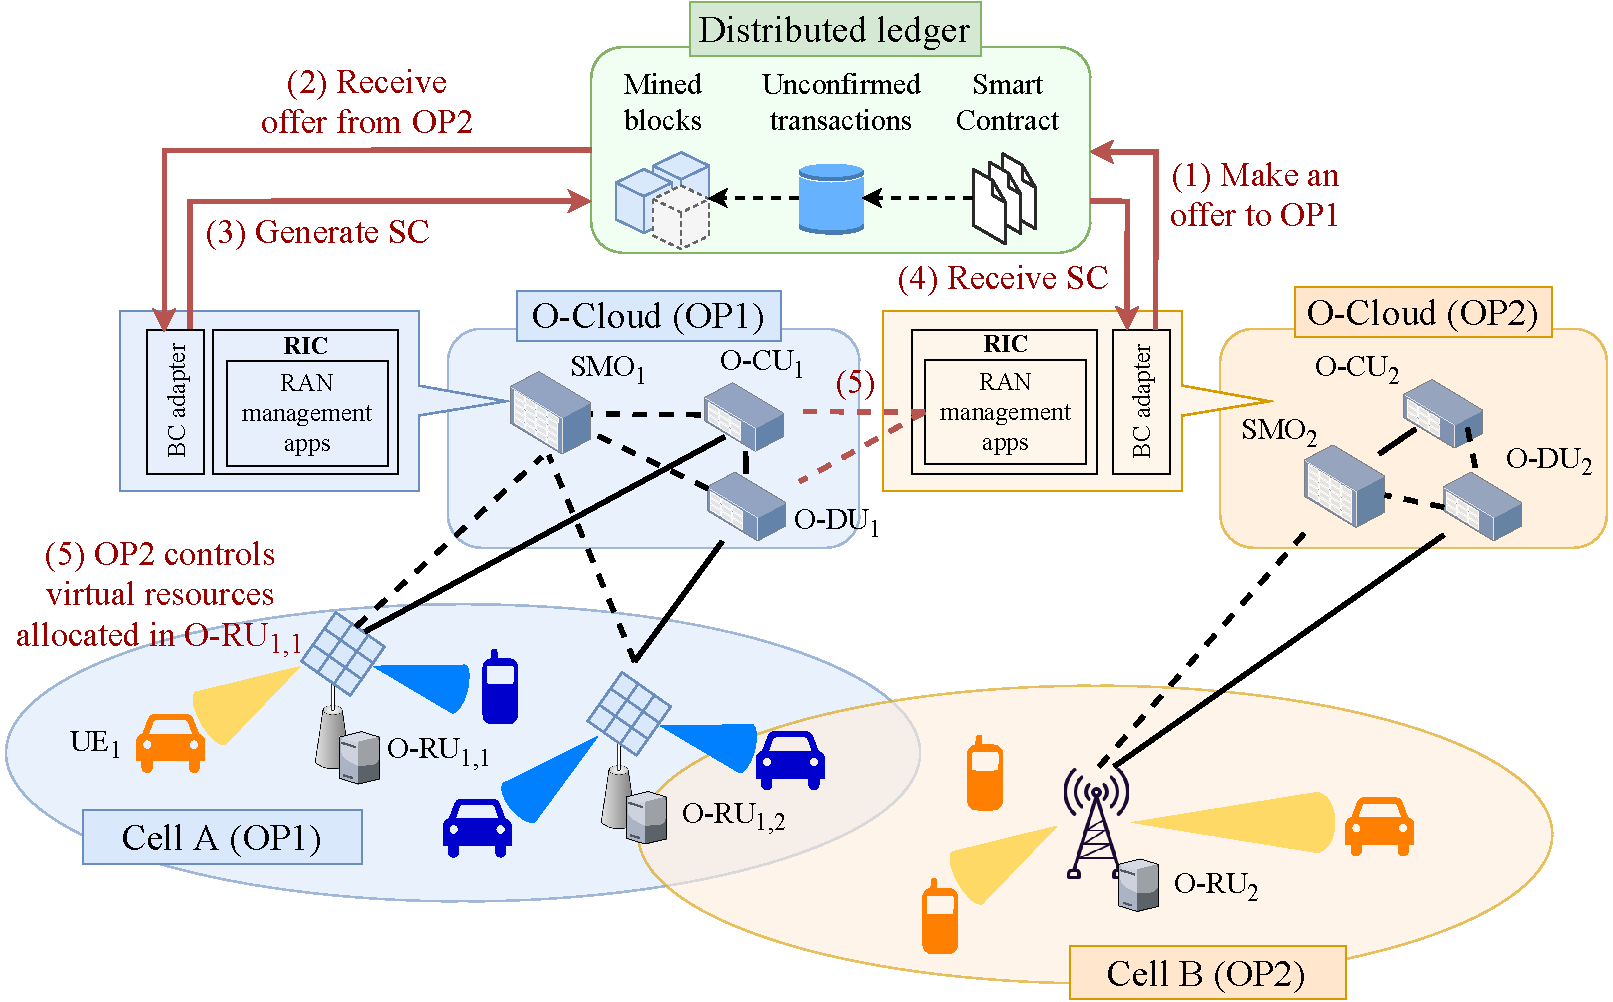
\includegraphics[width=\linewidth]{blockchain_ran-ecosystem}
\caption{BC-enabled RAN sharing ecosystem.}
\label{fig:blockchain_ecosystem}
\end{figure}

The use of virtualization in the RAN sector allows Mobile Operators (OPs) to deploy custom RAN functions composed of Virtual Network Functions (VNFs) to meet specific user demands and minimize network investments. The novel architecture proposed by O-RAN generates new opportunities related to offering, distribution and execution of VNFs by other OPs. Traditional and virtual operators or service providers can quickly contract and deploy VNFs from catalogues (i.e., marketplaces) to support the end users' demands. Operators with  available resources on their site can openly expose their service conditions and prices, so that any other user can observe the market and pick the more suitable infrastructure. In this case, competition is open, but quite static, as prices are not adapted to specific users' demands. Other strategies can be implemented to enable dynamic and real-time competitive resource trading, which favors lower prices, while meeting users' needs. 

Reverse auctions have been proposed in literature to enable flexible competition among providers~\cite{franco2019brain}. In a reverse auction, sellers compete for buyers and the auction winner is the one that provides the higher users' satisfaction in terms of price and offered service. This allows operators to monetize their infrastructure by receiving resource requests and giving sealed bids to offer requested resources for a price. After the bidding process, the auction decides the appropriate operator to host the requested resources. 

To support and provide trust for such auctions, we propose the introduction in O-RAN mnagement of Blockchain (BC) and Smart contracts (SC) technologies, since they offer immutable and permanent records, for interested parties to audit. The SC is used to describe the end user's requirements and allow for Service Level Agreement (SLA) enforcement. On top of the automation and efficient network management proposed by NG-SON and O-RAN, BC removes the need for costly intermediaries (e.g. a bank, credit rating agency, regulatory entity) and enables unprecedented levels of transparency, information sharing, with the potential for high savings. In addition, it reduces the delay required to establish agreements facilitating a real dynamicity in RAN resource sharing. 

%5G has also proposed additional novel features aimed at limiting capital and operational expenditures, like network slicing or spectrum sharing, which are changing traditional wireless paradigms: 1) cloudification, NFV, and network slicing concepts have transformed the network infrastructure deployment, 2) spectrum sharing has progressed towards a virtualization of the spectrum asset ownership, altering its valuation and utility. These changes are triggering the emergence of a new sharing economy in the telecom sector, where: 1) the model of exclusive spectrum rights is moving towards shared spectrum; 2) the concept of owning and controlling the end-to-end network infrastructure is getting obsolete, and the trend is to leverage the existing infrastructure as much as possible.

%In this context, we argue that 6G needs sustainable network management strategies, enabling intelligent environments, where a huge variety of users’ relationships are available. This vision moves forward with respect to 1) the traditional static auction-based spectrum allocation, which divides the spectrum into licensed, unlicensed and shared bands, and 2) the current time and effort required to define agreements among parties for sharing resources, based on legal contracts, and on the involvement of third party intermediaries (e.g. a bank, credit rating agency, regulatory entity). These static and administratively heavy approaches prevent innovation, automation and efficient, sustainable use of resources. 

%In this paper we propose to move forward with respect to the current time and effort required to define agreements among parties for sharing resources, based on legal contracts, and on the involvement of third party intermediaries (e.g. a bank, credit rating agency, regulatory entity). These static and administratively heavy approaches prevent innovation, automation and efficient, sustainable use of resources. 
%We focus then on an economically driven RAN management, and we propose an architecture based on O-RAN, where a dynamic secondary market exists. This secondary market allows network users to optimally choose between capital investment and resource use on a continuous basis, and not only at the time of auction, contract signature, or network deployment. 
%Resource trading allows for the establishment of dynamic and competitive markets, where new actors, besides the traditional operators appear, democratizing and decentralizing the telecom market. 
%To enable this vision, the proposed architecture includes Blockchain (BC) technology, which becomes the third technology, besides NG-SON and novel RAN Architectures, to facilitate automation and efficient network management. BC establishes trust mechanisms that can remove the need for costly intermediaries and enable unprecedented levels of transparency, information sharing, and has the potential for high savings in mobile networks. In addition, it reduces the delay required to establish agreements facilitating a real dynamicity and fluidity of resource sharing. 

%More specifically, we foresee a 6G scenario where users are not necessarily bound by a fixed contract to an MNO, but can advertise the need for a service in a BC through a smart contract defining the specifics of the requested service. Different actors like traditional MNO, Virtual MNO, or service providers participate in a reverse auction to offer the best service at a competitive price to a UE, which can select the most adequate provider based on its own utility function and current needs. The automation of this exchange is enabled through a BC, where the miners can be spread through the scenario and associated to UEs, Access Points (APs), gNBs. 

In this context, we propose a BC enabled RAN sharing for 6G scenario where O-RAN is the baseline architecture. OPs dynamically sublease their resources to others to capitalize on available infrastructure, and allow other OPs to increase coverage and delivered capacity. Each OP is allowed to optimally choose between capital investment and resource use on a continuous basis, and not only at the time of RAN sharing contract signature, or network deployment. This use case is of topical importance due to the openness provided in 4G and 5G (to be sustained and further motivated in 6G) and the emergence of new MVNO delivering specialized services to increasing niche markets. Dynamic resource trading allows for the establishment of new competitive markets, where new actors, besides the traditional OPs appear, democratizing and decentralizing the telecom market. An example is Google Fi, which offers cost-effective phone plans with added value such as cloud storage or discounts in Google-brand phones.

The introduction of BC in the network management has, however, also well documented limitations \cite{FWilhelmi_PIMRC}. Maintaining a BC among a wide number of peers incurs heavy costs in computation, power, energy consumption and memory usage. 
To run a BC in a mobile network, also represents a high traffic overhead for the network itself due to the distribution of blocks across the BC participants. The introduction of delay to perform the mining process is another aspect that affect the network performance, the users' perception of the service, and the stability of the BC itself, since the higher the introduced latency, the more likely are the forking events. The target of this paper is then to first propose a BC-enabled O-RAN based architecture for 6G, and then to evaluate some advantages and disadvantages incurred by the introduction of the BC in O-RAN management, in terms of delay for service establishement as a function of number of participating operators, BC block size the block timeout. The rest of this paper is organized as follows: Section~\ref{section:related_work} introduces the concept of BC technology and briefly overviews its standardization and application to communications systems. Then, Section~\ref{section:architecture} describes the proposed architectural framework for BC-enabled RANaaS, which potential benefits and challenges are pointed out in Section~\ref{section:results}. Section~\ref{section:conclusions} concludes the paper with final remarks.

%Another key aspect which has not been investigated is the impact of the communication transmission delay on a BC run over a wireless network. This is because available BC deployments have been up to now uniquely designed for stable and wired communication environments. Considering these challenges, we evaluate the impact of the wireless environment, where BC users and miners need to compete for wireless resources to broadcast transactions. In particular, the longer it takes to distribute transactions and blocks in the blockchain network, the more this will be unstable, unreliable and susceptible to forks. 

% Blockchain is particularly useful to provide trust and validity to the procedures of selling/buying resources among multiple stakeholders (thanks, to immutability/transparency/security aspects of blockchain). The blockchain is therefore in charge of storing relevant information from the auction procedures (e.g., bids, transactions, price, fulfillment of services, etc.).

% Operators can sublease their resources to others for delivering services to UEs, increasing the coverage area, or even improving the delivered capacity. This use case is of topical importance due to the emergence of new MVNOs delivering specialized services to increasing niche markets.\footnote{See, for instance, the case of Mexican MVNO that has been recently created by a popular \textit{Youtuber}, which exemplifies the shifting trends and the falling of market-entry barriers in telecommunications: \url{https://pillofon.mx/}. Another prominent example is Google Fi (\url{https://fi.google.com/}, which offers cost-effective phone plans with added value such as cloud storage, discounts in Google-brand phones, etc.)}

%%%%%%%%%%%%%%%%%%%%%%%%%%%%
%% TUTORIAL SECTION ON BC AND NETWORK/RAN SHARING
%%%%%%%%%%%%%%%%%%%%%%%%%%%%
\section{A Primer on BC-enabled Network Sharing in Cellular Networks}
\label{section:related_work}

A BC is a type of distributed ledger technology (DLT) compiling transactions in blocks that are sequentially and criptografically chained one after the other. The record of the transactions is maintained across several computers which communicate through a peer-to-peer (P2P) network. Nodes enabled to add transactions to the BC are referred to as miners. The miners organize the unconfirmed transactions into blocks and append them to the BC, after achievement of cosensus. The consensus mechanism is an advanced cryptographic technique executed by all the participants of the BC, which allows validation of the new block without the need to rely on a central trusted central authority. This automation of transactions is one of the most valuable features of BC for trading in future mobile networks. BC was firstly introduced with the cryptocurrency Bitcoin~\cite{nakamoto2019bitcoin}. Successively, with the introduction of smart contracts i.e., computer programs that run on top of the BC and self-execute the terms of a contract when specific conditions are met, BC's applications started appearing in multiple domains~\cite{cai2018decentralized}.

The advent of BC raises issues of interoperability both at a technical level (how various technical interfaces talk to each other) and at a semantic level (how information exchanged is understood by the various parties involved), which needs to be addressed by standardization activities. Important standardization organizations such as the International Telecommunication Union (ITU) and the European Telecommunications Standards Institute (ETSI) have been working on BC technology and released important documents with respect to BC terminology, use cases, ecosystem, or architectural aspects (see, e.g.,~\cite{ITU1400,etsi2020permissioned}). Apart from that, we find other initiatives like the European Blockchain Observatory and Forum, an open project to accelerate BC innovation within the EU, or the standardization of some DLT properties by W3C or Open Timestamps. To obtain a broader view on the standardization of BC, we refer the interested reader to~\cite{konig2020comparing}.

%through various Study Groups and the Focus Group on the Application of Distributed Ledger Technology, since 2017. Besides, ETSI has recently released important documentation on Permissioned Distributed Ledger~\cite{etsi2020permissioned} and foreseen the utilization of smart contracts through a use case whereby NFVI services are delivered on-demand~\cite{virtualisation2018release}.

Many industries are already introducing BC and the list of potential use cases is rich. In the telecom sector, much research work has been ongoing in the area of BC-based Internet of Things (IoT) and Beyond 5G (B5G). BC has been widely envisioned to manage network sharing and resource trading of network slices to provide service to vertical applications~\cite{xu2020blockchain}. In particular, BC may become the basis of a decentralized and transparent platform for multi-party negotiation between the increasing number of stakeholders (e.g., VNF providers, multiple administrative domains) involved to offer an E2E network slice. A survey on BC applications for 5G can be found in~\cite{nguyen2020blockchain}.

The advertisement of services and automation of administrative negotiations in the form of an open marketplace may become a fundamental piece of a new ecosystem where providers operate from the cloud, to trade resources, \textit{as-a-service}. Service Level Agreements (SLA) are defined by smart contracts, and guaranteed by a proactive Artificial Intelligence (AI) based management. In the area of RAN, novel transformative architecture like O-RAN are moving in this direction, and we argue that the integration of BC will allow the implementation of a \textit{RAN-as-a-service vision}. In one of its defining documents \cite{ORAN}, the {O-RAN} Alliance introduces different use cases, associated to multiple technical areas like load/traffic management, radio, vertical management, and RAN sharing and slicing. In this area, identified use cases of interest are RAN slice SLA Assurance, multi-vendor slices, NSSI Resource Allocation, Dynamic Spectrum Sharing (DSS), BBU pooling to achieve RAN elasticity and RAN sharing. 

In this paper, we focus in the RAN sharing use case. RAN sharing is a widely adopted method used by OPs to cost-efficiently increase their coverage and services. 5G networks deployments also rely on RAN sharing for new RAN build out. RAN sharing arrangements emerge when two OPs agree to work together to capitalize on each others’ network assets. The introduction of BC technolgies in this context can automate, accelerate, and secure the definition of the relationship with a well defined SLA for trade of resources. Key Performance Indicator (KPI) monitoring will be implemented through AI functionalities, embedded in O-RAN architecture, which allows to enforce meaningful SLAs. 
%In the context of {O-RAN}, multiple OPs share the same {O-RAN} infrastructure and remote configuration is allowed through O1, O2 and E2 interfaces. %Specifically it is proposed that Operator A makes available its {O-RAN} infrastructure and hosts the virtual RAN functions of a second Operator B, which can remotely manage them via its RIC and through E2 remote interface.

In \cite{xu2021ran}, the authors introduced a BE-RAN architecture taking O-RAN baseline for the work, to conduct zero-trust mutual authentication over the unique BC-enabled routers, and switches functions with the identification exchanged over the BC. The main novelty proposed by \cite{xu2021ran} is to introduce BC to decentralize RAN security aspects, in opposite to the current centralized solutions based on PKI authetication and third-party trust. Different contributions in literature target the vision of BC to facilitate resource trading in the RAN segment. In \cite{maksymyuk2020blockchain}, the authors showed that static spectrum allocation forces OPs to increase the price of their services, which makes the OPs less competitive and results in negative profits. Taking this into account, the work proposed a protocol for BC-based spectrum trading in 5G/6G networks, where ledgers with different access privileges are managed. This allows to define a new paradigm whereby OPs adjust their prices and services according to the expected demand, while UEs select the option maximizing their utility at every moment. The authors compared a semi-persistent approach with dynamic and AI-based one. The best solution results the dynamic one, which was shown to incur in high overhead of the BC due to the high number of transactions. However, the specific increment in overhead was not studied. Finally, the work in \cite{togou2020dbns} described an architecture that facilitates the dynamic leasing of resources among network operators to support cross-domain services. The cornerstone of this architecture is a brokering layer, which relies on a BC-based bidding system to request resources and evaluate resource provisioning offers. 

%%%%%%%%%%%%%%%%%%%%%%%%%%%%
%% ARCHITECTURE
%%%%%%%%%%%%%%%%%%%%%%%%%%%%
\section{Architectural Framework for BC-enabled RAN Sharing}
\label{section:architecture}
We study how the RAN sharing process proposed for the O-RAN architecture can be improved to become dynamic and autonomous by the introduction of BC. We first introduce the basics on O-RAN and then discuss the proposed added blocks and their role.

\subsection{O-RAN Architecture}
The O-RAN Alliance was born in February 2018 to continue the evolution of 3GPP RAN architecture in areas like non-public networks, self-organized networks and integrated access and backhaul.
Its major tenat is to define open interfaces between the elements implemented in general purpose hardware. It is the first standard to enable multi-vendor RAN, and RAN virtualization, thus favoring efficient splits over the protocol stack for network slicing purposes. This flexibility allows to bring in new radio players and gives plenty of opportunities to operators to optimize deployments for specific performance requirements at much better cost. 

\begin{figure*}[ht!]
\centering
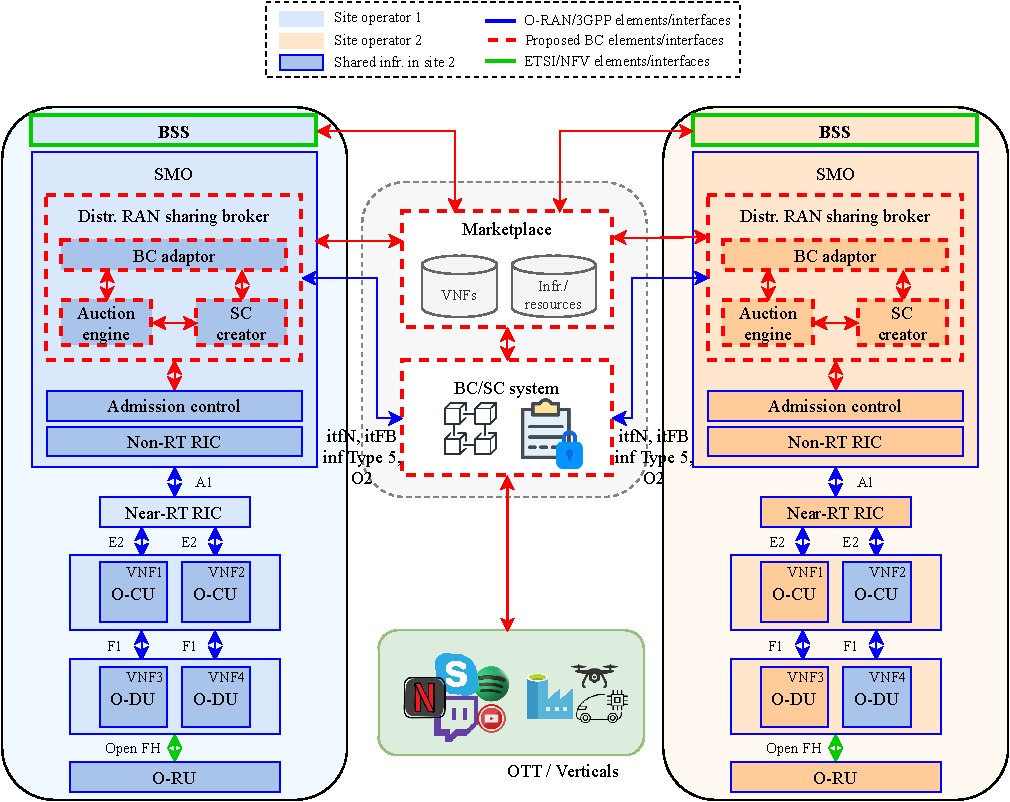
\includegraphics[width=0.75\textwidth]{functionalarchitecture2.pdf}
\caption{Functional BC-enabled O-RAN architecture.}
\label{fig:functionalarchitecture}
\end{figure*}

The O-RAN-based architecture is shown in Fig.~\ref{fig:functionalarchitecture}. It includes all the modules in the figure which are marked in blue (modules marked in red are later described in next subsection and are our proposal to support a BC-enabled architecture), and is based on the original 3GPP proposal in TS 38.401. These main modules are: System Management and Orchestration (SMO), O-CU (O-RAN Centralized Unit), O-DU (O-RAN Decentralized Unit), O-RU (O-RAN Radio Unit) and RICs (Radio Intelligent Controller). These modules are all deployed as Virtual Network Functions (VNF) or containers, and the interfaces them (depicted in blue in Fig.~\ref{fig:functionalarchitecture}) are defined by O-RAN in \cite{ORAN2}.  
\begin{itemize}
    \item \textbf{SMO:} The SMO, similar to other architectures based on ETSI NFV's, provides a variety of network management functionalities. In the context of O-RAN architecture and for RAN functionalities, it oversees all the orchestration, management and automation aspects. It includes Fault, Configuration, Accounting, Performance, Security (FCAPS) support for O-RAN functions, such as installation, configuration, or performance, fault, and file management. In addition, it includes the newly introduced non Real-Time (non-RT) RIC for intelligent RAN optimization. These functionalities are supported by newly introduced interfaces such as A1, O1 and O2.
    %
    \item \textbf{O-CU:} The O-CU hosts the gNB protocols of Radio Resource Control (RRC), Service Data Adaptation Protocol (SDAP) and Packet Data Convergence Protocol (PDCP), and is connected to the O-DU via F1-C and F1-U interfaces, for control and data planes respectively. The O-CU controls operation of multiple O-DU over midhaul interfaces. The split architecture enables different distributions of protocol stack between O-CU and O-DU, depending on the midhaul availability and the network design. %Functions like mobility and session management are handled by this logical node. 
    %
    \item \textbf{O-DU:} The O-DU hosts the Radio Link Control (RLC), the Medium Access Control (MAC) and PHY-high layers of the gNB, and is connected to the O-RU via the Open Fronthaul interface. This node includes a subset of the eNB/gNB functions, depending on the functional split option, and its operation is controlled by the O-CU.
    %
    \item \textbf{O-RU:} The O-RU is the radio unit handling the digital front-end and hosts the PHY-low and RF of the gNB. 
    %
    \item \textbf{RIC:} O-CUs are controlled by the RIC modules, newly introduced by {O-RAN}, the non-RT RIC and the near-real time RIC (near-RT RIC), supporting tasks with more or less than 1 s latency, respectively. Through these modules, the {O-RAN} architecture strives the industry to introduce embedded intelligence and artificial intelligence based RICs. RICs are based on software apps to orchestrate and manage the RAN. Applications like mobility management, admission control, and interference management are available as apps on the RIC, which enforces network policies to the radio segment. Non-RT RIC is implemented inside the SMO and includes service and policy management, RAN analytics and model-training for the Near-RT RIC. The trained model is managed by the SMO for deployment and is received by the near-RT RIC through A1 interface. The near-RT RIC uses the E2 interface to collect information at UE and cell basis and perform self-optimization tasks across the heteorogeneous RAN (e.g. formed by macros, Massive MIMO, small cells, etc.).
\end{itemize}
O-RAN has studied different options for CU/DU/RU deployment, including location in regional/edge clouds, or operator specific sites. The so called \textit{scenario B} is the initial priority of {O-RAN}. Here, O-CU and O-DU are located together in an edge cloud, while the O-RU is located in proprietary cell site. 

%\begin{figure}[ht!]
%\centering
%\includegraphics[width=\columnwidth]{oran_architecture.png}
%\caption{Original O-RAN architecture \cite{ORAN}.}
%\label{fig:oran_architecture}
%\end{figure}


\subsection{BC-enabled O-RAN}
We propose to enrich the O-RAN architecture with the inclusion of new functional blocks for the specific purpose to offer the opportunity of automatic, dynamic sharing of RAN resources through BC services. The functional architecture is depicted in Fig.~\ref{fig:functionalarchitecture}. The new proposed modules are depicted in red. The example shown in the figure represents a RAN sharing use case, where two traditionl OPs interact, and one of them requests resources to be leased to another OP. This use case is extendible to the case of virtual OPs, and to other OTT service providers and verticals requesting RAN resources. The introduction of BC technolgies in this context can automate, accelerate and secure the RAN sharing start-up phase between OP i and OP j to define the relationship with a certain service level agreement (SLA) for trade of resources. Remote configuration of instantaited VNFs in the host infrastructure of OP i is allowed through O1, O2 and E2 interfaces. Specifically it is proposed that OP j makes available its {O-RAN} infrastructure and hosts the virtual RAN functions of a second OP i, which can remotely manage them via its RIC and through E2 remote interface. Performance monitoring is implemented during the running phase through AI functionalities offered by RIC modules, which allows to ensure SLA is fulfilled and enforced. 

The proposed architecture includes different additions to the O-RAN baseline architecture, like the Business Support System (BSS) (in yellow), inhereted from European Telecommunications Standards Institute (ETSI)-NFV architecture, for the operator to deliver product, customer, and revenue management (billing). The SMO, besides the already introduced non-RT RIC, includes the admission control functionality that decides whether new VNF can be leased on the site infrastructure and feeds this information back to the newly introduced \textit{distributed RAN sharing broker}, depicted in red. In addition, we propose to introduce the concept of a \textit{marketplace}, where OPs can opt to advertize the infrastructure they are willing to offer, a BC/SC system, and a set of new interfaces: 1) an SMO internal interface for communication between the admission control and the RAN sharing broker; 2) different broker interal interfaces across its elements; 3) an interface between the BSS and the BC/SC system. The interface between the SMO and the BC/SC system reuses already available interfaces proposed by O-RAN and 3GPP by 3GPP or O-RAN, i.e. O2, Itf-N, Itf-B and Type~5 interface. Vertical industries and OTT providers interact with the BC and the OPs providing infrastructure through the so called Service Capability Exposure Function (SCEF).

The \textit{Distributed RAN sharing broker} is the entity that manages and offers RAN VNFs. The concept of broker has been previously introduced in~\cite{samdanis2016network} for network slicing, thus serving as a management point to gather requests from multiple parties such as MVNOs, OTTs or vertical providers, and providing admission control. The blocks that conform the distributed RAN sharing broker are:
\begin{itemize}
    \item \textbf{SC creator}: The SC creator is in charge of mapping requirements and preferences into a SC format, so that other operators are informed about the selected service from a marketplace, or obtain information to participate with bids to an auction process. The SC defines the SLA that needs to be monitored during the running phase, including information such as the type of resources, required QoS, the service duration, or tolerance indicators. Once the SC is compiled and distributed, the Auction engine is triggered, if an auction phase is required to select the preferred service.
    \item \textbf{Auction engine}: is the component in charge of handling the auction process. For the requesting OP, the auction engine is in charge of collecting the bids submitted by the OPs participating to the auction, selecting the winner based on precise algorithm for end users' expected satisfaction, triggering the communication between the own SMO and the SMO of the selected OP in order to start the instantiation of requested VNFs. The auction starts after the SC is deployed, and is concluded after a predefined period depending on time, reception of a certain number of bids, achievement of a price target, etc. For the candidate OPs, the auction engine is in charge of defining the bid to be submitted based on internal bid algorithms depending on business variables, available resources, proce for unit of resurces, special discount, and expected return of investment. During each auction process, bids and decisions are securely recorded inside the BC for distributed decisions related to auctions and future audits.
    \item \textbf{BC adaptor}: the BC adaptor is the entity in charge of handiling the communication with the BC, registering the OP to it, etc.
\end{itemize}

The BC in the proposed architecture is a private BC that uses SC, only operators deploying a RAN sharing broker can join the BC. We propose two different flows of the proposed architecture, as depicted in Fig.~\ref{fig:functionalarchitectureflowdiagram}:
\begin{itemize}
    \item \textit{Marketplace-oriented}: All OPs with VNFs, infrastructure and resources to offer advertize them with specific prices in a catalog (i.e., marketplace), where other OP, MVNO, OTT providers or verticals can select the desired service. To participate in the marketplace, the OP registers the information of interest (e.g., available resources, price of resources) in the BC. OP$_i$, interested in leasing a VNF from another OP providing infrastructure, accesses the marketplace to acquire one. After selecting a sharing provider OP$_j$, the SC creator in the RAN sharing broker of OP$_i$ prepares a SC defining the SLA, based on the offer identified in the marketplace. This is distributed in the BC and received by the BC adaptor of OP$_j$, which translates the SC into requirements and sends them to the admission control of the SMO for evaluation. If the request is accepted, a VNF is instantiated in OP$_j$'s infrastructure to be remotely configured (during the configuration phase) by OP$_i$ through the open interfaces defined in O-RAN. During the running phase, the SLA is monitored through RICs at OP$_i$ site. If need for update of resources is identified by the SMO, an update service request is sent to the RAN sharing broker and a new SC is prepared by the SC creator, which is then registered in the BC and analyzed by OP$_i$'s admission control. If the service can be modified, the request is accepted.
    %
    \item \textit{Auction-oriented}: In this variant of the procedure, the selection of the serving OP i is done by means of an auction procedure, which is expected to better satisfy the end users' in terms of price and delivered service. The OP j interested in leasing VNFs/infrstructure/resources from another OP defines the requirements and desired price for the needed resources and send them to the SC creator of the RAN sharing broker of OP j. The SC creator prepares a SC, which is distributed through the BC. Other OPs interested in offering for lease their resources and infrastructure, evaluate availability through admission control functionality, and if the resources are available, participate in the auction offering a bid through the auction engine. The auction engines distribute the bids from the candidate OPs through the BC. The auction engine of OP j collects the bids and decides the target i to host the desired VNFs. From this moment this procedure is similar to the first case. The provisioning request is sent to the hosting OP, to the RAN sharing broker, and an instantiation request is sent to the orchestrator to be instantiated in the platform of site i. 
\end{itemize}

%\begin{figure*}[ht!]
%\centering
%\subfigure[Marketplace]{\includegraphics[width=\columnwidth]{flowdiagram_marketplace.pdf}\label{fig:2}} 
%\subfigure[Auction]{\includegraphics[width=.95\columnwidth]{flowdiagram_auction.pdf}\label{fig:1}} 
%\caption{Flow diagram of BC-enabled O-RAN functional architecture, for marketplace and auction oriented cases.}
%\label{fig:functionalarchitectureflowdiagram}
%\end{figure*}

\begin{figure}[ht!]
\centering
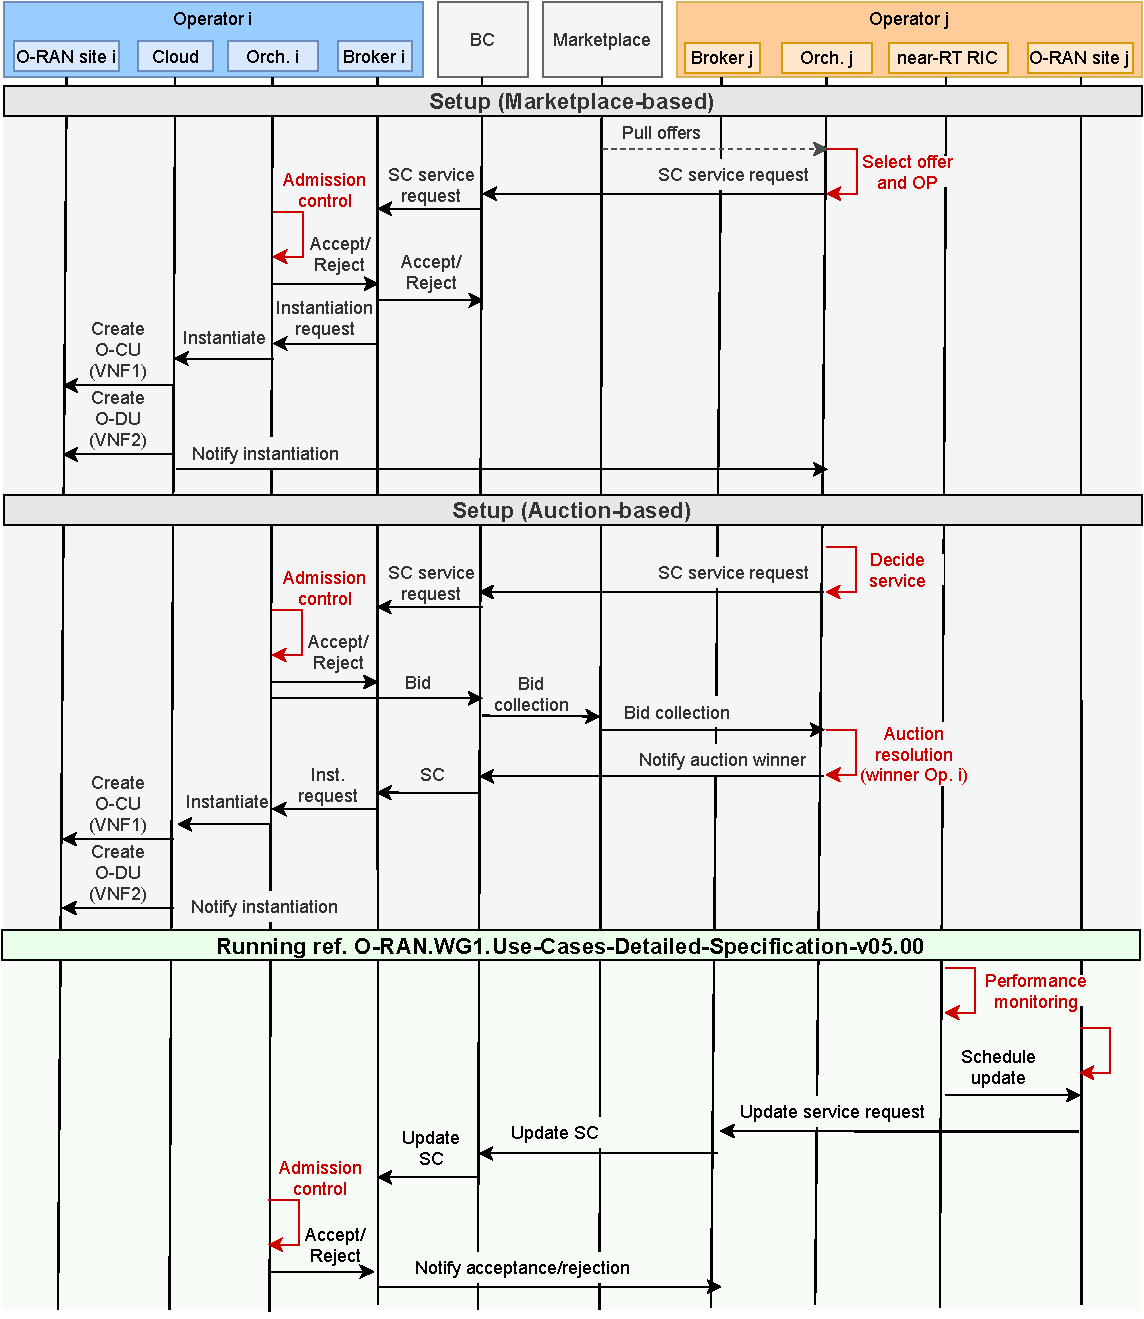
\includegraphics[width=1\columnwidth]{flowdiagram_complete.pdf}
\caption{Flow diagram of BC-enabled O-RAN functional architecture, for marketplace and auction-oriented cases.}
\label{fig:functionalarchitectureflowdiagram}
\end{figure}

%%%%%%%%%%%%%%%%%%%%%%%%%%%%
%% USE CASE
%%%%%%%%%%%%%%%%%%%%%%%%%%%%
\section{BC-enabled RAN sharing: opportunities and challenges}
\label{section:results}
The introduction of BC-enabled RAN sharing offers OPs new opportunities for new revenue incomes by capitalizing on available infrastructure. In this section, we analyze the different opportunities and challenges, as well as the trade-offs among them, of the proposed BC-enabled RAN sharing architectural framework. The most important opportunities offered by BC and SC to traditional RAN sharing are:
\begin{enumerate}
    \item \textbf{Automated management:} thanks to the introduction of SCs, it is possible to automate some of the procedures in RAN sharing. By removing long interactions with third parties in the negotiation for sharing resources, improved network management efficiency is expected.
    %
    \item \textbf{Resources efficiency:} through automated RAN sharing, resources can be fully harnessed by multiple parties, thus leading to higher network capacity, more coverage and, consequently, improved users' satisfaction.
    %
    \item \textbf{Competitiveness:} with the entry of new actors to the RAN sharing ecosystem, competitiveness is expected to be boosted, thus leading to further service diversification and additional possibilities to improve the network infrastructure. This is expected to attract more investments in the network.
    %
    \item \textbf{Auditablity:} the traceability of every interaction in a BC allows for improved trust and transparency in RAN sharing. This is an important aspect to take into account, considering the recent issues raised by, e.g., Ericsson warning on O-RAN security~\cite{boswell2020security}.
\end{enumerate}

Concerning the challenges, BC and SC systems have several well documented drawbacks to take into account when considering their inclusion in an established trading system. The salient challenges are: 
\begin{enumerate}
    \item \textbf{Communication overhead:} the communication among peer nodes and miners in BC introduces certain overhead that needs to be considered. The overhead increases with the number of participants and the duration of the requested services (accurate short-term requests vs long-term fixed contracts).
    %
    \item \textbf{Transaction confirmation latency:} the distribution of transactions and blocks across the BC determines the delay for instantiating RAN functions in the infrastructure prividers's platform. The transaction confirmation delay in a BC strongly depends on the adopted consensus mechanism (e.g., Proof-of-Work) and on the system arrivals. A detailed model to estimate the transaction confirmation latency based on those parameters in wireless blockchain networks can be found at~\cite{FWilhelmi_PIMRC}.
    %
    \item \textbf{Stability:} the stability of a BC is strongly related to the fork occurrences, which are a side effect of the distributed consensus mechanism. First, the performance of a BC may be jeopardized by high propagation delays. Specifically, the higher the delay, the higher the probablity of being susceptible to forks. Moreover, game-theoretical aspects may motivate selfish behaviors among miners (e.g., releasing a mined block at the appropriate time so that other mined blocks are invalidated), thus adding instability to the BC.
    %
    \item \textbf{Scalability:} given the nature of BC, whereby all the transactions need to be propagated and stored, an increase in the number of BC users and transactions can represent both a communication and a storage issue. Besides, BC is originally limited by the block size and the mining difficulty (see, e.g., the case of Bitcoin), thus limiting the effective transactions rate. 
\end{enumerate}

%Among these aspects, in this paper, and due to space constaints, we focus on the analysis of the delay between the service request and the instantiation of the VNF. For more analysis on the key challenges of BC/SC systems, the reader is referred to \cite{FWilhelmi_PIMRC}, where more details on fork probability, stability, scalability and overhead are given.

Now, we demostrate the superiority of proposed BC-enabled RAN sharing scheme in front of the no-sharing situation (i.e., static) situation. For that, Fig.~\ref{fig:performance} shows the potential performance gains achieved by the autonomous marketplace and auction-oriented sharing mechanisms in cellular random deployments containing up to 19~cells and 200~UEs.\footnote{\textit{For the sake of reproducibility and disclosure, all the source code is open and publicly available at \url{https://bitbucket.org/francesc_wilhelmi/blockchain_enabled_ran_architecture}, accessed on Jul. 31, 2021.}} In particular, we evaluate the UE capacity, based on the set of resources allocated to each user and its SINR, and the user satisfaction, based on the obtained service and the price paid for it. Besides, we show the efficiency of each approach, thus indicating the degree to which BS resources are harnessed. The efficiency is computed as the inverse of the difference between the load requested by users and the actual load at BSs.

\begin{figure}[ht!]
\centering
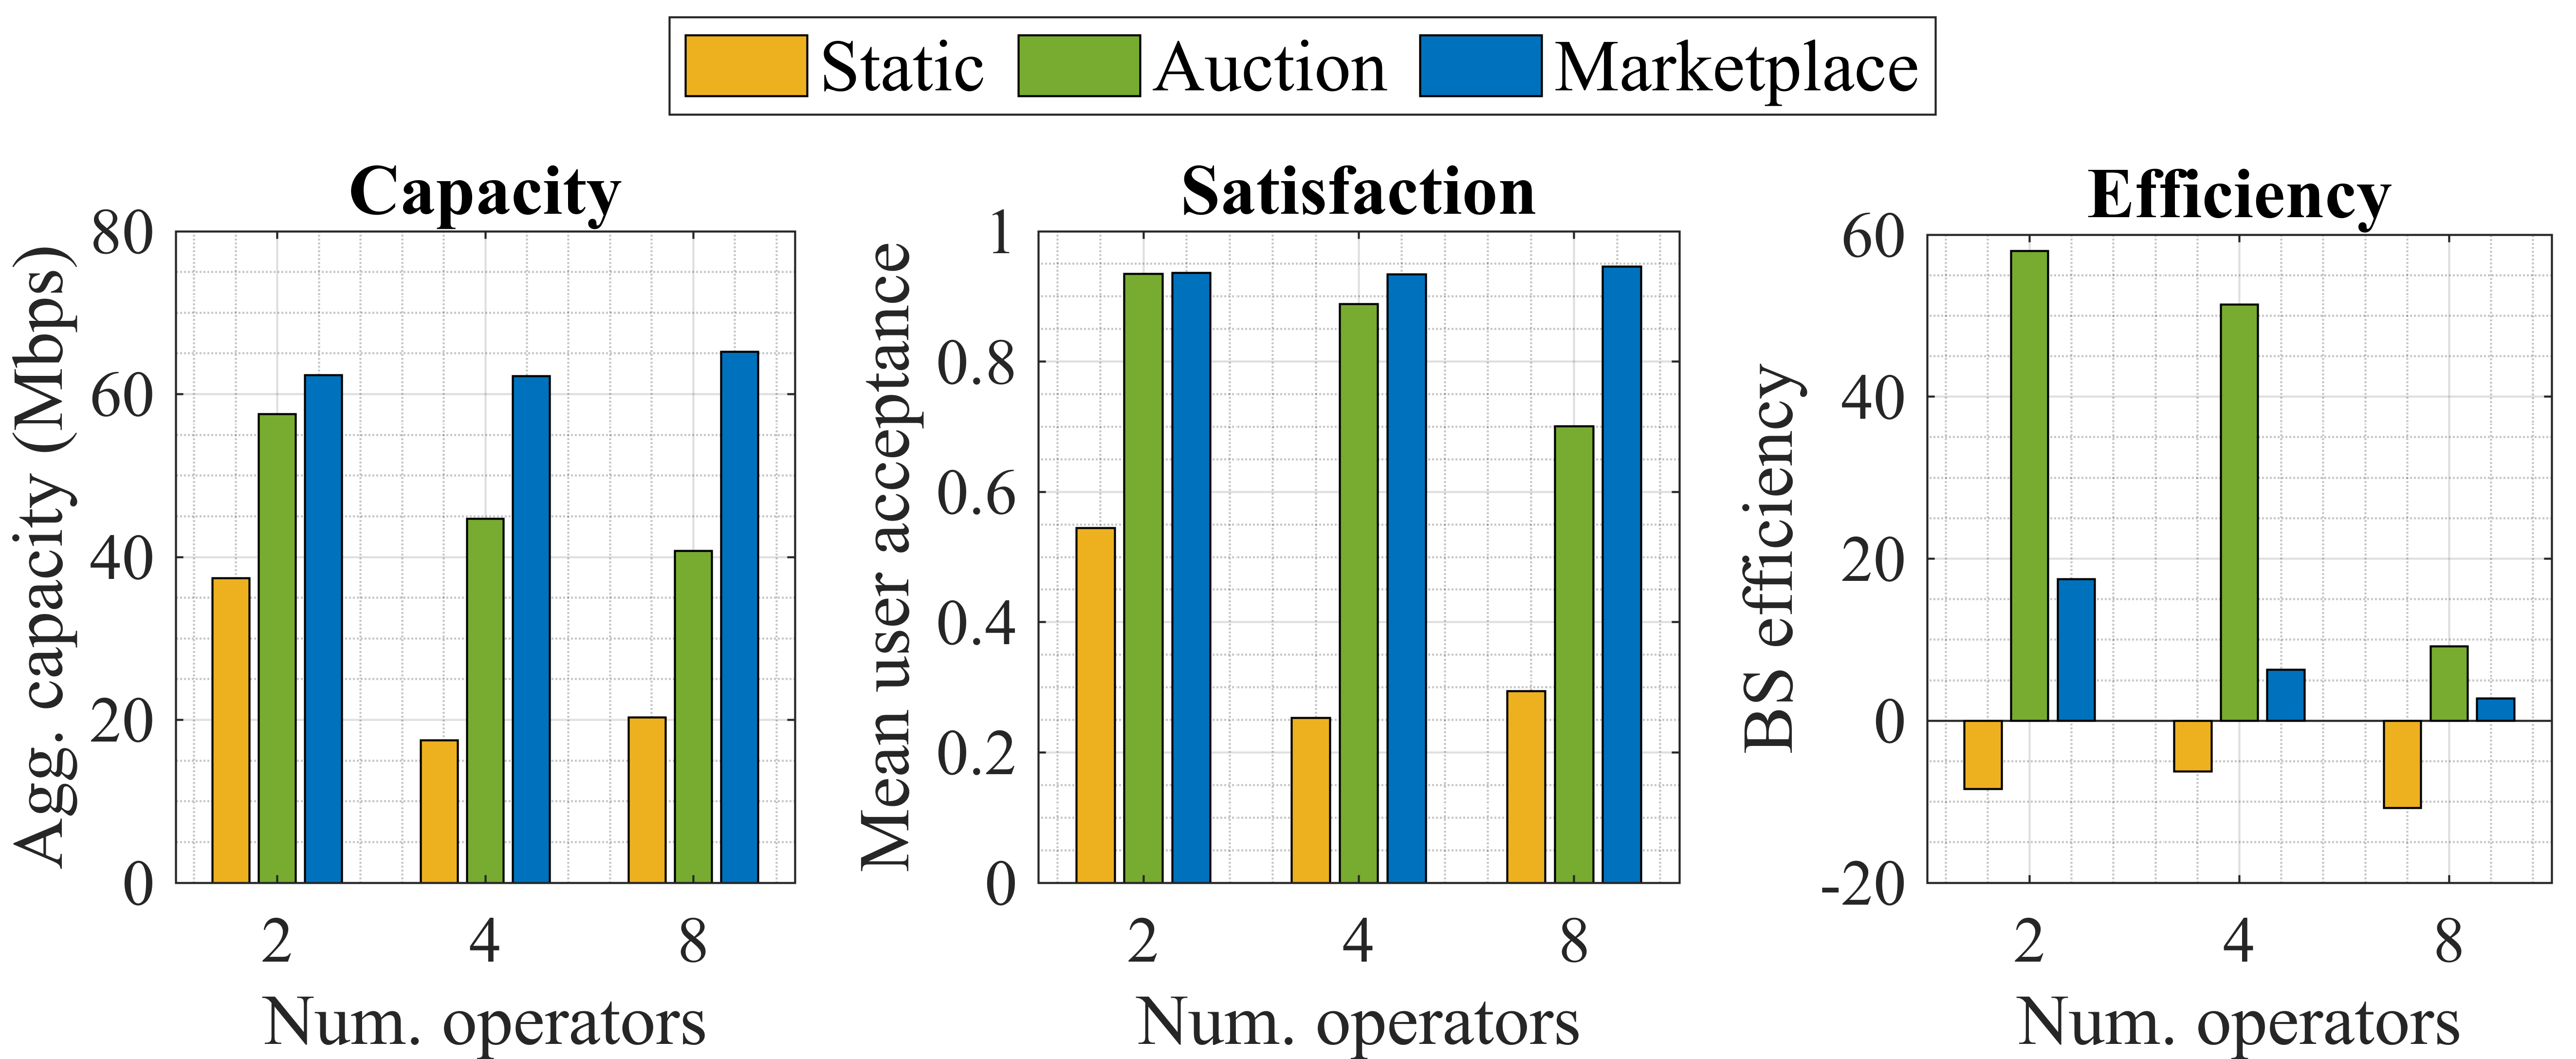
\includegraphics[width=1\linewidth]{performance_results.png}
\caption{UE performance and efficiency of the different BC-enabled RAN sharing mechansism compared to the static situation.}
\label{fig:performance}
\end{figure}

As shown in Fig.~\ref{fig:performance}, both BC-enabled auction and marketplace-based solutions outperform the static scenario (at which RAN resources are not shared) in terms of UE capacity (in the left of the figure) and satisfaction (in the middle of the figure). Automating the exchange of resources among operators is essential to improve the utilization of the same infrastructure resources, thus potentially leading to increased gains and profits. MNOs with underutilized infrastructure can obtain additional resources from MVNOs, who can access the market and obtain niche profits. Besides UE performance, the BC mechanisms lead to higher efficiency, being the auction-based the most efficient one.

Now, to showcase some of the implications of the BC, we focus on the overhead and the additional delay incurred by the proposed RAN sharing solution~\cite{ORAN}. We denote the delay between the service request and the instantiation of the VNF function in OP$_j$ infrastructure site by $T_{RAN,sh}$ and $T_{RAN,bc}$, which refer to the baseline O-RAN and the proposed BC-enabled RAN sharing procedures, respectively. In particular, $T_{RAN,bc}=T_{RAN,sh}+T_{BC}$, where $T_{BC}$ is the total time needed to define the SC with the agreed service and to distribute it through the BC. In the marketplace-oriented case, such a delay comprises the time for propagating the SC service request and automatically enforcing it based on marketplace offers, whereas the auction-based procedure also includes the distribution of bids over the BC. In Fig.~\ref{fig:delay_overhead}, we illustrate the delay ($T_{BC}$) and overhead incurred by both the auction and marketplace-based BC-enabled RAN sharing solutions. The results comprise different numbers of operators (2, 4, and 8), user requests ratio (1, 5, and 10 service requests per second), and block size values (from 3,000 to 30,000 bits).

\begin{figure}[ht!]
\centering
\subfigure[Delay]{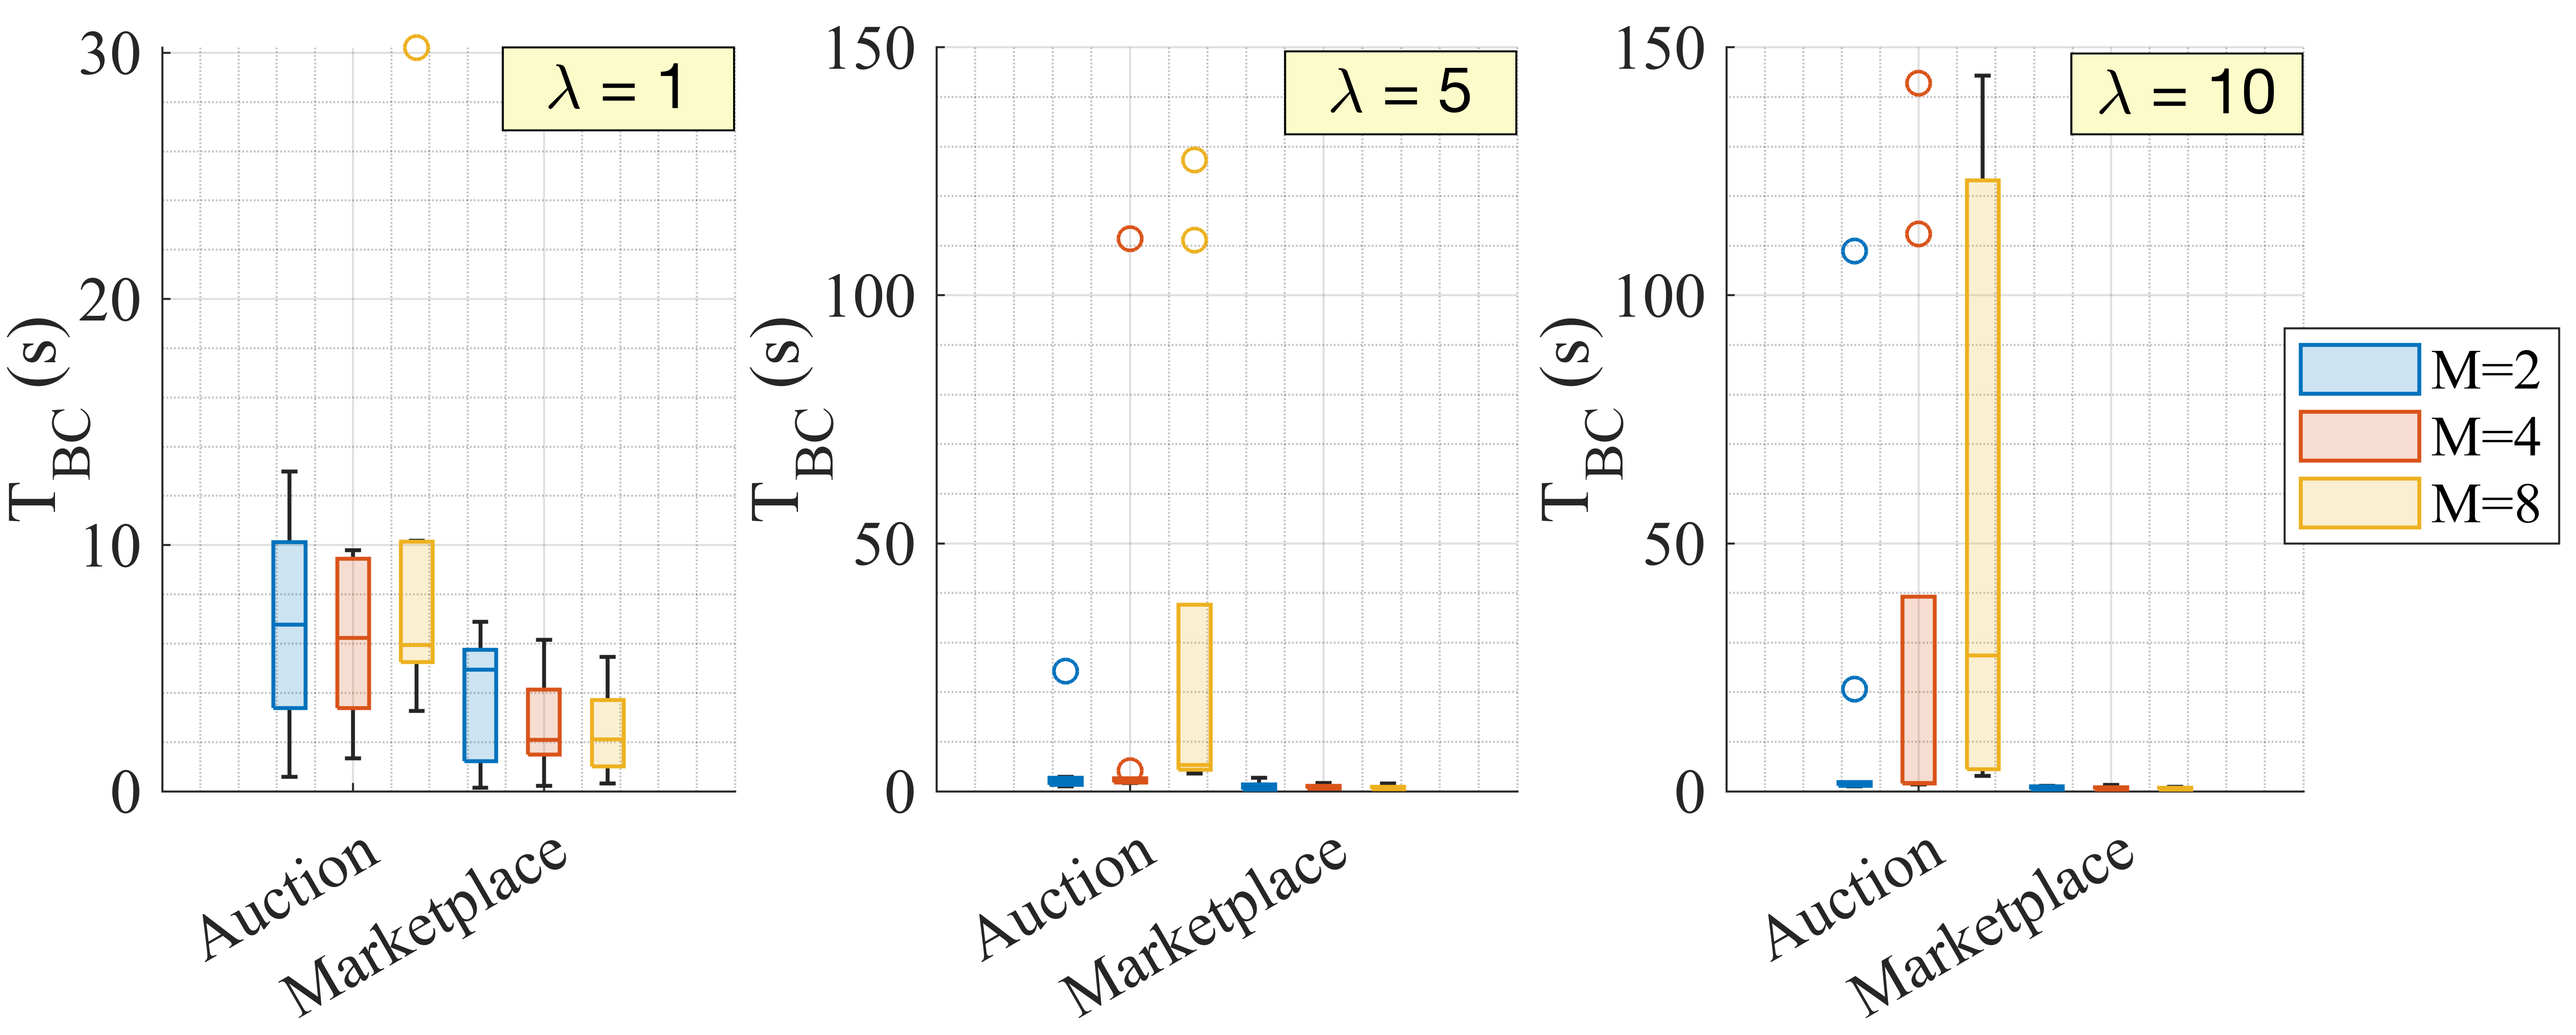
\includegraphics[width=\columnwidth]{boxplot_combined_delay.png}\label{fig:2}} 
\subfigure[Overhead]{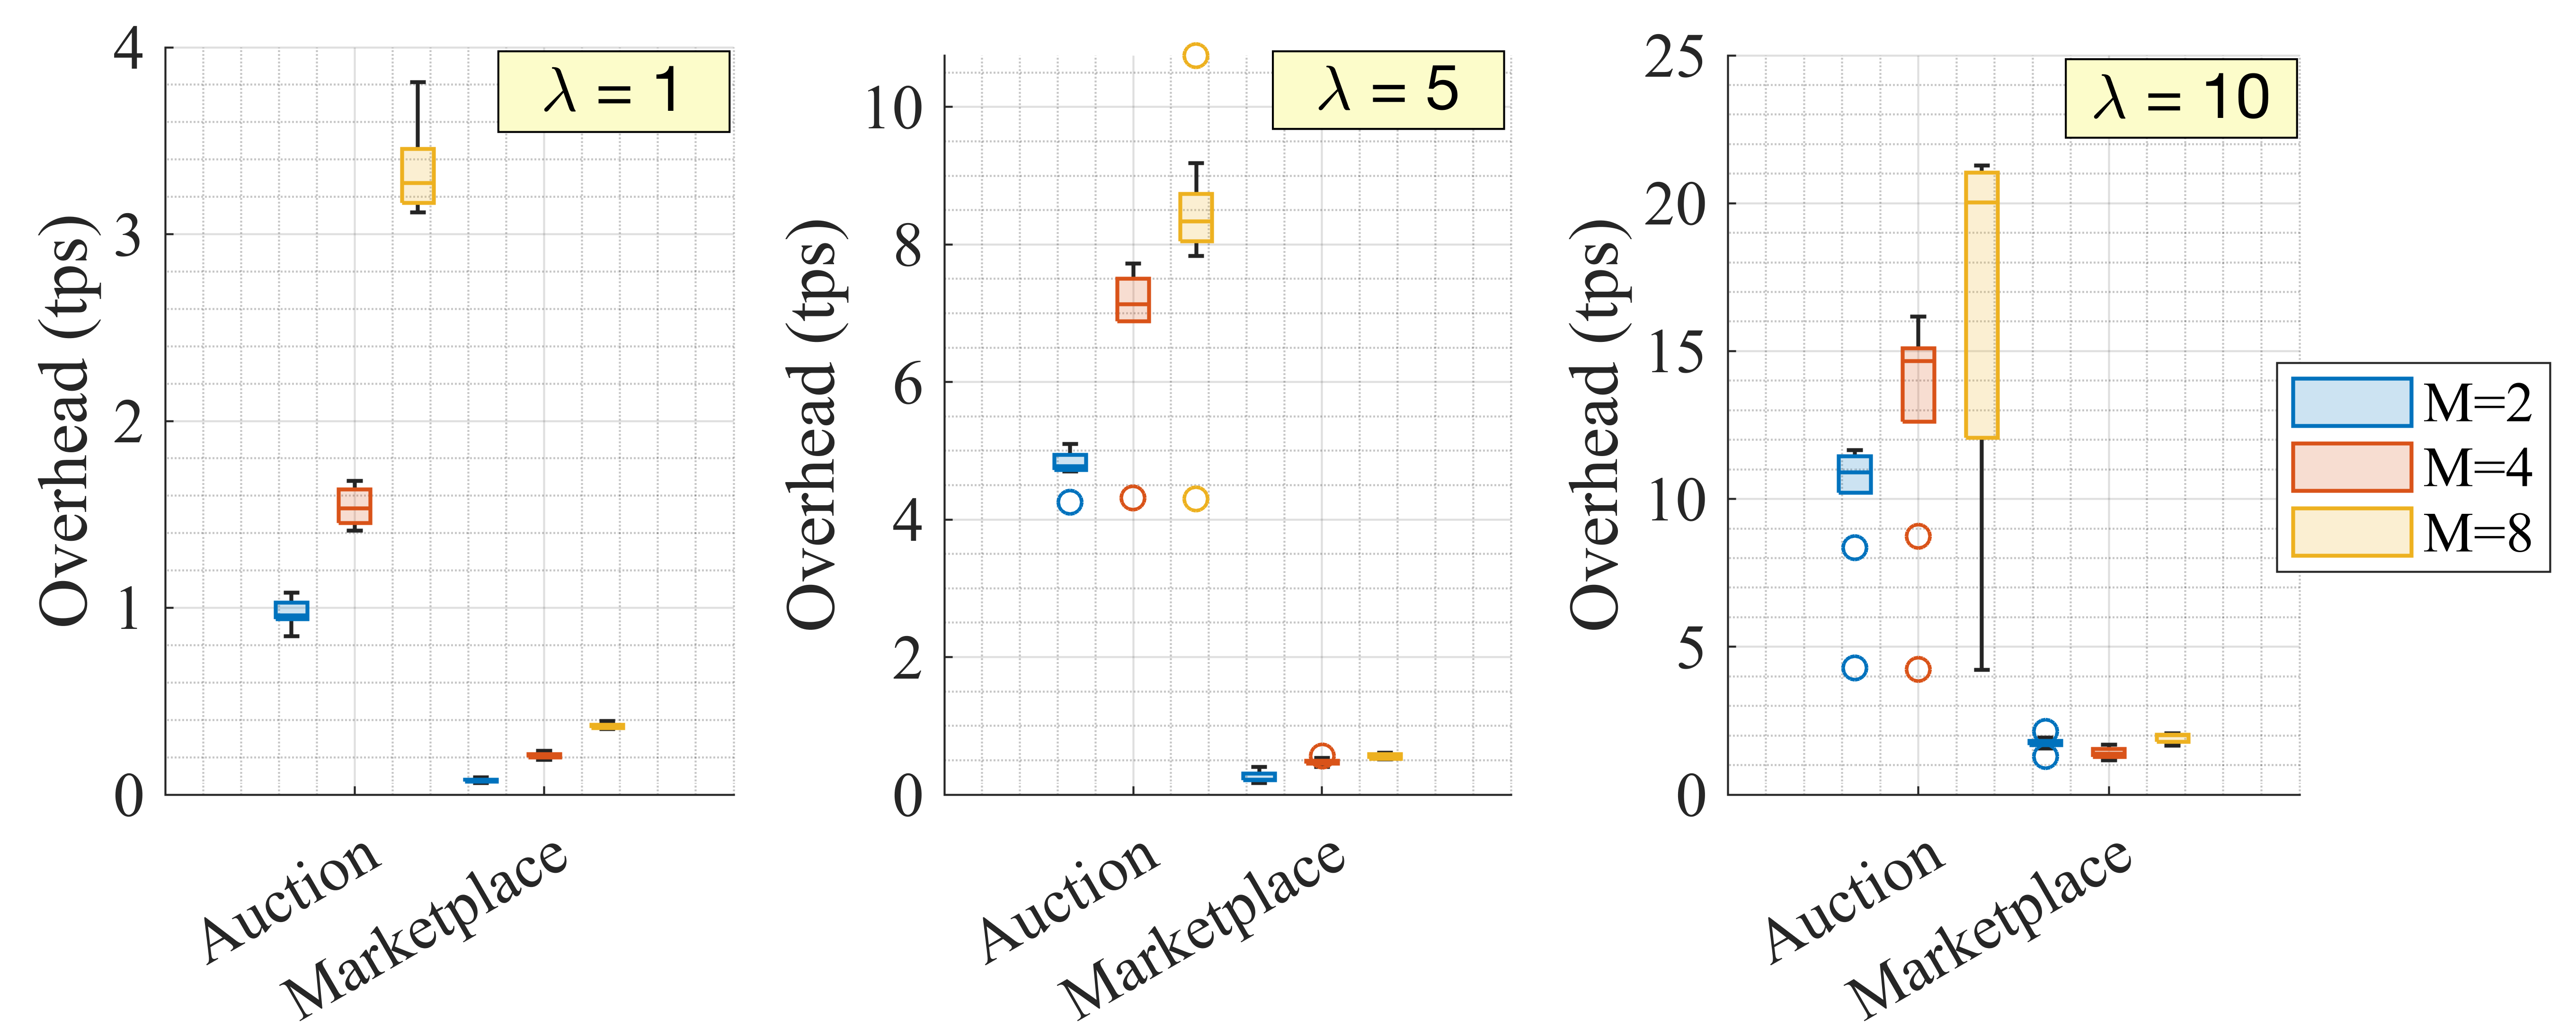
\includegraphics[width=\columnwidth]{boxplot_combined_overhead.png}\label{fig:1}}
%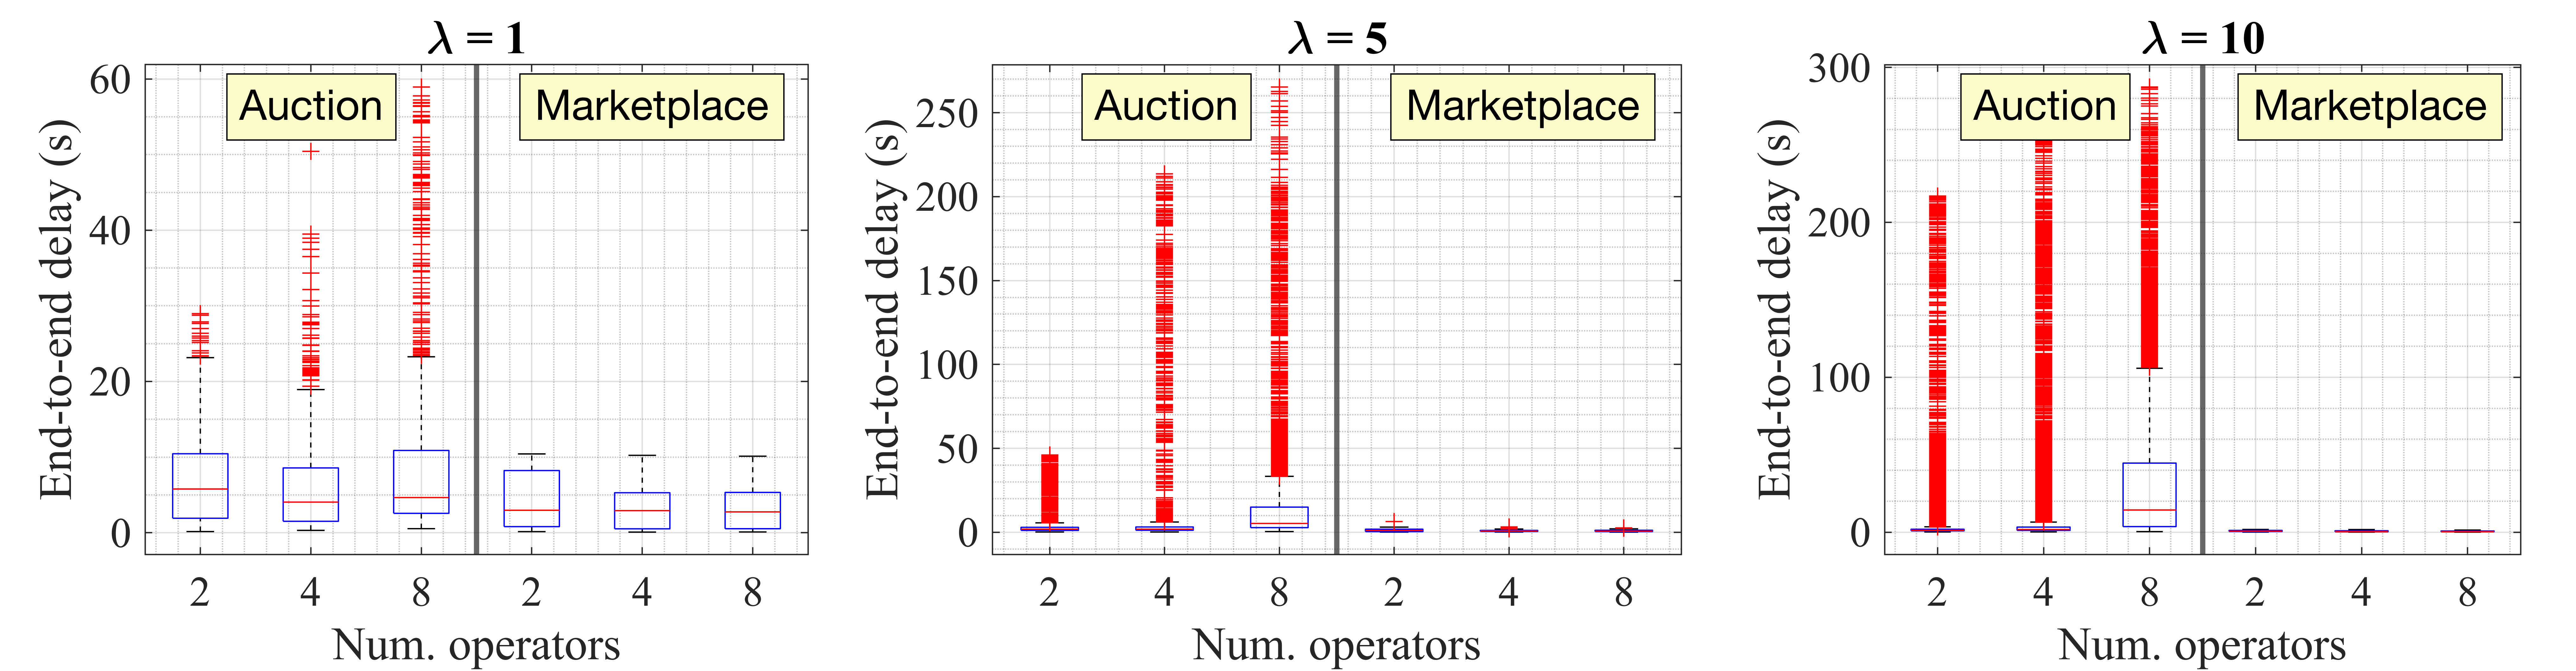
\includegraphics[width=.75\linewidth]{boxplot_all.png}
\caption{End-to-end delay and overhead incurred by the BC for both auction and marketplace-oriented RAN sharing solutions. Different block sizes, user arrival rates, and number of operators have been considered.}
\label{fig:delay_overhead}
\end{figure}

As illustrated, the auction-based mechanism leads to higher delay and overhead than the marketplace approach. The fact is that the auction leads to a higher number of BC transactions, which result from generating tailored service requests and auction bids. This property is exacerbated as the number of user arrivals increases and for a higher number of sharing operators. As for the marketplace option, a low delay and overhead are maintained for a different number of operators, thus becoming a cost-effective solution for automating RAN sharing procedures in future communications systems. Moreover, the delay incurred by the marketplace BC approach decreases with the number of user arrivals, which contributes to system efficiency. As for the block size (included in each boxplot), a higher variability is observed in the auction-based approach, which is more susceptible to performance changes for different BC parameters. A more detailed analysis on the impact of multiple BC parameters (e.g., block size, user arrivals rate, mining timeout, fork probability) on wireless networks can be found in~\cite{FWilhelmi_PIMRC}.

%The detailed and analytical computation of the delay  $T_{BC}$ can be found in \cite{FWilhelmi_PIMRC}, where we have modeled and validated a discrete-time Markov model to capture the expected delay incurred by the BC. %Among these aspects, in this paper, and due to space constraints, we focus on the analysis of the delay between the service request and the instantiation of the VNF. For more analysis on the key challenges of BC/SC systems, the reader is referred to \cite{FWilhelmi_PIMRC}, where more details on fork probability, stability, scalability, and overhead are given.

%%%%%%%%%%%%%%%%%%%%%%%%%%%%
%% CONCLUSIONS
%%%%%%%%%%%%%%%%%%%%%%%%%%%%
\section{Conclusions}
\label{section:conclusions}
The virtualization and softwarization of network functions provided by 5G will disrupt the way RAN resources are shared. In this context, the O-RAN Alliance is contributing to the development of standards on \textit{intelligent, open, virtualized, and fully interoperable mobile networks}, thus building a sharing ecosystem for future communications. However, a set of issues arise when defining SLAs among operators and multiple parties. To address that, we envision the utilization of Blockchain technology, which is expected to provide trust and traceability to the automation of network sharing. In particular, we have proposed a novel O-RAN-based BC-enabled architecture and defined new components and procedures to carry out two automated RAN sharing mechanisms, namely auction and marketplace-oriented. Besides, we have demonstrated the potential of the proposed architecture through simulation results, thus showing the superiority of the auction and marketplace approaches in terms of capacity, user satisfaction, and efficiency. Moreover, we have provided some insights on the impact of adopting BC for network sharing, especially regarding additional delay and overhead.

\section*{Acknowledgment}
This work was funded by the IN CERCA grant from the Secretaria d'Universitats i Recerca del departament d'Empresa i Coneixement de la Generalitat de Catalunya, and partially from the Spanish MINECO grant TEC2017-88373-R (5G-REFINE) and Generalitat de Catalunya grant 2017 SGR 1195.
	
\ifCLASSOPTIONcaptionsoff
\newpage
\fi
	
\bibliographystyle{IEEEtran}
\bibliography{bibliography}

% if you will not have a photo at all:
\begin{IEEEbiographynophoto}{Francesc Wilhelmi}
(fwilhelmi@cttc.cat) holds a Ph.D. in Information and Communication Technologies (2020), from Universitat Pompeu Fabra (UPF). Previously, he obtained a B.Sc. degree in Telematics Engineering (2015) and an M.Sc. in Intelligent and Interactive Systems (2016), also from the UPF. He is currently working as a postdoctoral researcher in the Mobile Networks department at Centre Tecnològic de Telecomunicacions de Catalunya (CTTC). He is also a teaching assistant at the UPF since 2015 and a course instructor at Universitat Oberta de Catalunya (UOC) since 2020.
\end{IEEEbiographynophoto}
%
\begin{IEEEbiographynophoto}{Lorenza Giupponi}
(lorenza.giupponi@cttc.es)
\end{IEEEbiographynophoto}

\end{document}